\section{From real world to two-dimensional images}

Images exist on a 2D plane, while the real world is three-dimensional, leading to a reduction of information compared to the original subject.
This reduction is a result of perspective projection, which exhibits the following characteristics: nonlinearity, lack of shape preservation, and failure to maintain length ratios.

Using the triangle equality, we can express this perspective projection as:
\[x=f \dfrac{X}{Z} \qquad y=f \dfrac{Y}{Z}\]
To minimize information loss, one effective approach is to capture an image of a planar scene on a plane that is parallel to the image plane. 
This requires that:
\[Z=Z_0=\textnormal{constant}\]
\begin{figure}[H]
    \centering
    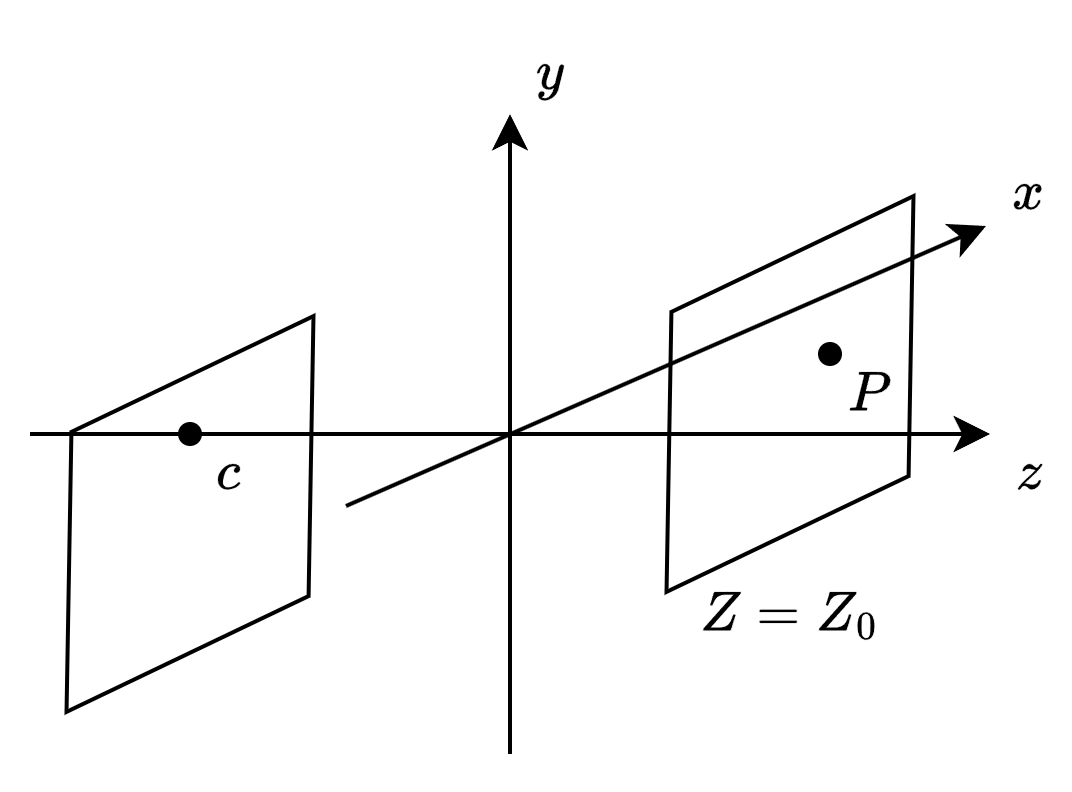
\includegraphics[width=0.5\linewidth]{images/Z0.png}
\end{figure}
In this scenario, the only difference between reality and the projection is a uniform downscaling, while other dimensions are preserved, yielding:
\[x=f \dfrac{X}{Z_0}=kX \qquad y=f \dfrac{Y}{Z_0}=kY \]